\section{Predictive models}\label{sec:models}

The predictive statement asks for two estimates at the start of a month. Both models here are ordinary linear regressions fitted to every row that has the needed values, and both are judged on those same rows. Each uses three predictors I chose from the correlation matrix, all known before the month starts. I recorded the direction I expected for each slope before either model was fitted.

\subsection*{The regression problem: free play per \$100 wagered}

\textbf{Target and predictors.} The target is free play deducted per \$100 wagered. The predictors are last month's free play per \$100 (the strongest correlation, \V{r_fp_prior}), the number of months the sportsbook has been active (\V{r_fp_months}), and operator type, which enters as 1 for a commercial sportsbook and 0 for a tribal one.

\textbf{Fitted equation.}
\begin{center}
free play per \$100 $=$ \V{m1_b0} $+$ \V{m1_b1} $\times$ (last month's free play per \$100) $-$ \V{m1_b2} $\times$ (months active) $+$ \V{m1_b3} $\times$ (commercial)
\end{center}

\begin{table}[H]
\centering\small
\caption{Model 1 estimates (\V{m1_rows} sportsbook-months). Source: output/tables/model1\_estimates.}\label{tab:m1}
% Written by scripts/08_report_numbers.R from output/tables. Do not edit by hand.
\begin{tabular}{@{}p{0.55\linewidth}rrr@{}}
\toprule
Term & Estimate & Standard error & p value \\
\midrule
Intercept (a tribal operator with every numeric predictor at zero) & 3.2356 & 0.4271 & under 0.001 \\
Prior month: free play per \$100 wagered & 0.4975 & 0.0243 & under 0.001 \\
Months the operator has been active & -0.0323 & 0.0099 & 0.001 \\
Commercial operator (1 = commercial, 0 = tribal) & 0.1308 & 0.4354 & 0.76 \\
\bottomrule
\end{tabular}

\end{table}

\textbf{What each slope means.} Table~\ref{tab:m1} gives the estimates. A sportsbook that deducted \$1 more of free play per \$100 last month tends to deduct about \V{m1_prior_cents} cents more per \$100 this month, holding months active and operator type fixed. I expected less, not more: heavy free play carries over from one month to the next. Each extra month a sportsbook has been active goes with about \V{m1_months_cents} cents less free play per \$100, or about \$\V{m1_months_year} less per year, holding the other two fixed. I expected it to go up; the result fits the launch pattern in Figure~\ref{fig:age}. A commercial sportsbook is predicted to deduct \$\V{m1_com_dollars} more per \$100 than a tribal one with the same history, but that estimate is small next to its standard error of \$\V{m1_com_se_dollars}, so the model does not tell the two types apart.

\textbf{Fit.} The model accounts for \V{m1_r2_pct}\% of the differences in free play per \$100 (R-squared \V{m1_r2}). Its typical miss, the root mean squared error, is \$\V{m1_rmse} per \$100, which is large beside a median of \$\V{fp_median}. A few months drive that figure. Figure~\ref{fig:m1a} and Figure~\ref{fig:m1b} show that \V{m1_within5_n} of the \V{m1_rows} predictions (\V{m1_within5_pct}\%) land within \$\V{def_within}, while \V{m1_above10} months came in more than \$\V{def_big_miss} above the prediction, the largest by \$\V{m1_largest_miss}; \V{m1_above10_lump} of those \V{m1_above10} are flagged lump-deduction months. \V{m1_left_out} rows were left out: \V{m1_no_prior} because the sportsbook has no month before it in the data and \V{m1_missing_value} because this month's or last month's free play value is blank.

\begin{figure}[H]
\centering
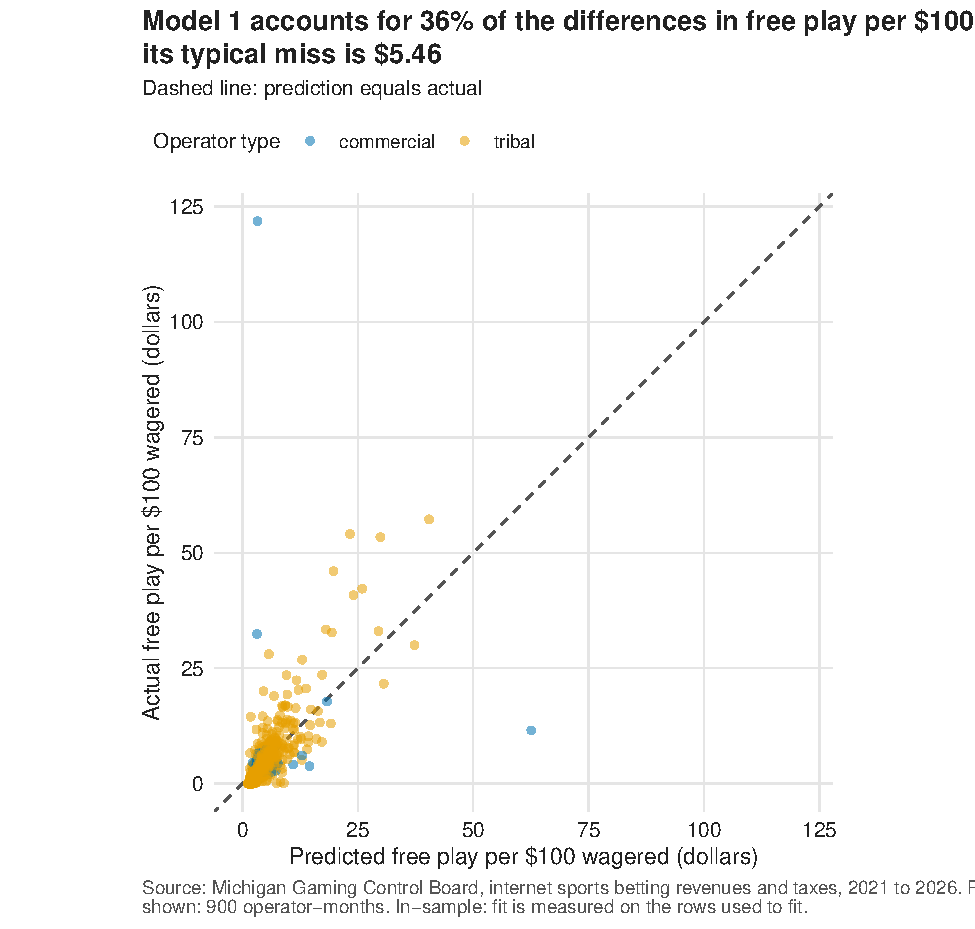
\includegraphics[width=0.74\linewidth]{figures/fig_m1_predicted_vs_actual.pdf}
\caption{Model 1: predicted against actual free play per \$100 wagered. Source: Michigan Gaming Control Board; \V{m1_rows} sportsbook-months, the rows used to fit.}\label{fig:m1a}
\end{figure}

\begin{figure}[H]
\centering
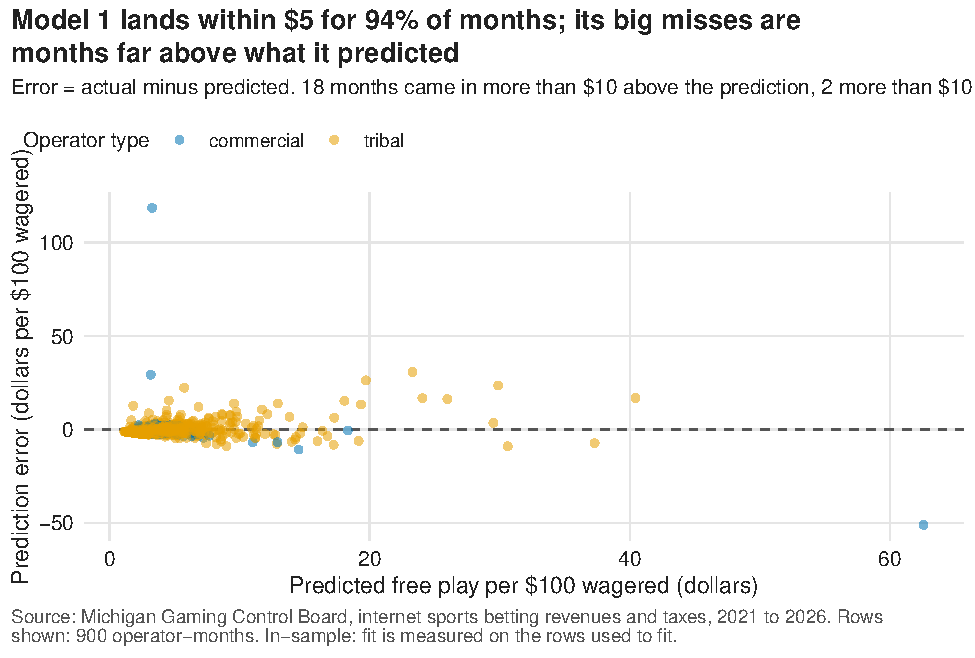
\includegraphics[width=0.92\linewidth]{figures/fig_m1_errors_vs_predicted.pdf}
\caption{Model 1: prediction errors against predicted values. Source: Michigan Gaming Control Board; \V{m1_rows} sportsbook-months, the rows used to fit.}\label{fig:m1b}
\end{figure}

\subsection*{The classification problem: paying no state tax}

\textbf{Target and predictors.} The target is 1 if the sportsbook paid no state tax or payment in the month and 0 if it paid something. A linear regression on a 0-and-1 target is a linear probability model, and its prediction is read as the probability of a yes. The predictors are whether the sportsbook paid no tax last month (\V{r_nt_prior}), the size of last month's wagering on a log scale, where one unit is a tenfold increase (\V{r_nt_priorsize}), and operator type.

\textbf{Fitted equation.}
\begin{center}
probability of no tax $=$ \V{m2_b0} $+$ \V{m2_b1} $\times$ (paid no tax last month) $-$ \V{m2_b2} $\times$ (log of last month's dollars wagered) $-$ \V{m2_b3} $\times$ (commercial)
\end{center}

\begin{table}[H]
\centering\small
\caption{Model 2 estimates (\V{m2_rows} sportsbook-months). Source: output/tables/model2\_estimates.}\label{tab:m2}
% Written by scripts/08_report_numbers.R from output/tables. Do not edit by hand.
\begin{tabular}{@{}>{\raggedright\arraybackslash}p{0.55\linewidth}rrr@{}}
\toprule
Term & Estimate & Standard error & p value \\
\midrule
Intercept (a tribal operator with every numeric predictor at zero) & 0.6532 & 0.1085 & under 0.001 \\
Prior month: paid no state tax (1 = yes, 0 = no) & 0.7353 & 0.0222 & under 0.001 \\
Prior month: size (log10 of dollars wagered) & -0.0771 & 0.0156 & under 0.001 \\
Commercial operator (1 = commercial, 0 = tribal) & -0.0084 & 0.0289 & 0.77 \\
\bottomrule
\end{tabular}

\end{table}

\textbf{What each slope means.} Table~\ref{tab:m2} gives the estimates. A sportsbook that paid no state tax last month has a predicted probability of paying none this month that is about \V{m2_prior_points} percentage points higher than one that paid, holding last month's size and operator type fixed. Each tenfold increase in last month's dollars wagered goes with a probability about \V{m2_size_points} percentage points lower, holding the other two fixed. Both are the directions I expected. A commercial sportsbook's predicted probability is \V{m2_com_points} percentage points lower than a tribal one's with the same history, with a standard error of \V{m2_com_se_points} points, so the model shows no difference between the types once last month's tax status and size are held fixed. The gap between the types in Section~\ref{sec:eda} (\V{tri_notax_pct}\% against \V{com_notax_pct}\%) goes with those two things in this model, not with type itself.

\textbf{Fit.} R-squared is \V{m2_r2}. Calling a prediction of \V{def_cutoff} or more a yes, Table~\ref{tab:class} shows the model is right for \V{m2_correct_n} of \V{m2_rows} months (\V{m2_correct_pct}\%). Always guessing the more common outcome, that tax was paid, would be right \V{m2_baseline_pct}\% of the time. The model misses in both directions: \V{m2_no_yes} months it called no-tax paid tax, and \V{m2_yes_no} months it called tax-paying paid none. \V{m2_outside} predictions (\V{m2_outside_pct}\%) fall outside 0 to 1, \V{m2_below0} below 0 and \V{m2_above1} above 1, with a largest value of \V{m2_max}; they are reported as they are (Figure~\ref{fig:m2}). \V{m2_left_out} rows were left out because the sportsbook has no month before it in the data.

\begin{table}[H]
\centering\small
\caption{Model 2: predicted against actual at the \V{def_cutoff} cutoff. Source: output/tables/model2\_classification\_table.}\label{tab:class}
% Written by scripts/08_report_numbers.R from output/tables. Do not edit by hand.
\begin{tabular}{@{}lrrr@{}}
\toprule
  & Predicted yes (0.5 or more) & Predicted no (under 0.5) & Total \\
\midrule
Actual: paid no tax (yes) & 394 & 43 & 437 \\
Actual: paid tax (no) & 50 & 419 & 469 \\
Total & 444 & 462 & 906 \\
\bottomrule
\end{tabular}

\end{table}

\begin{figure}[H]
\centering
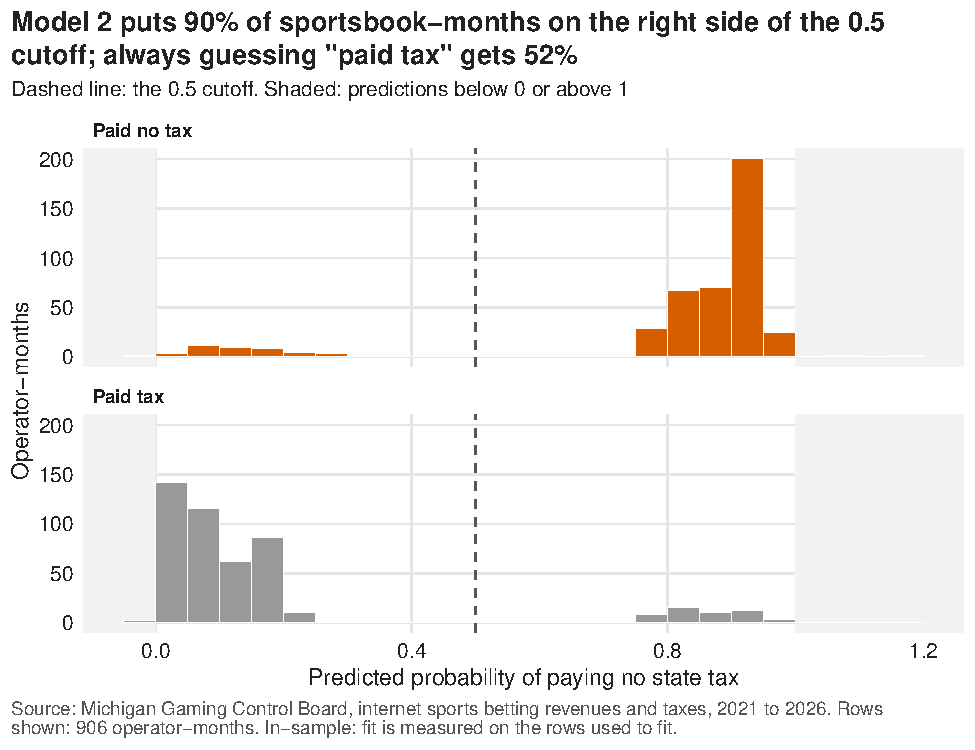
\includegraphics[width=0.92\linewidth]{figures/fig_m2_predicted_probability.pdf}
\caption{Model 2: predicted probability of paying no state tax, shown separately for months that did and did not. Source: Michigan Gaming Control Board; \V{m2_rows} sportsbook-months, the rows used to fit.}\label{fig:m2}
\end{figure}

\subsection*{Three cases}

Table~\ref{tab:cases} gives both predictions for three sportsbooks the Board might ask about. None of the values lies outside the range seen in the data. A large commercial sportsbook four years in is predicted to deduct \$\V{case1_m1} per \$100 and has a \V{case1_m2_pct}\% predicted probability of paying no tax. A small tribal sportsbook that paid no tax last month is predicted at \$\V{case2_m1} and \V{case2_m2_pct}\%. A tribal sportsbook in its fourth month with heavy free play is predicted at \$\V{case3_m1} and \V{case3_m2_pct}\%.

\begin{table}[H]
\centering
\caption{Scenario predictions from both models. Source: output/tables/model\_scenarios.}\label{tab:cases}
\resizebox{\linewidth}{!}{% Written by scripts/08_report_numbers.R from output/tables. Do not edit by hand.
\begin{tabular}{@{}p{0.27\linewidth}rrllrrrl@{}}
\toprule
Case & Free play last month (\$ per \$100) & Months active & Type & No tax last month & Wagered last month (\$) & Model 1 (\$ per \$100) & Model 2 (probability) & Beyond the data? \\
\midrule
1. Large commercial sportsbook, four years in, paid tax last month & 4.00 & 48 & commercial & no & 100,000,000 & 3.81 & 0.0278 & No \\
2. Small tribal sportsbook, five years in, paid no tax last month & 5.00 & 60 & tribal & yes & 1,500,000 & 3.78 & 0.9122 & No \\
3. Tribal sportsbook in its fourth month, heavy free play, paid no tax last month & 9.00 & 4 & tribal & yes & 3,000,000 & 7.58 & 0.8889 & No \\
\bottomrule
\end{tabular}
}
\end{table}

Both models describe association in these months, not cause. Fit was measured on the rows the models were fitted to, so these figures are a best case; on new months the models would probably do somewhat worse.
